\documentclass[ECP,preprint]{ejpecp}
% The finite-size shape transition of coin-turning walks.
% The class ejpecp is in TeX Live. Build: pdflatex s4_note.tex, three times.

\usepackage[shortlabels]{enumitem}

% ---------- notation macros (the class provides theorem, lemma,
% proposition, corollary, definition, example and remark, numbered within
% sections) ----------
\newcommand{\Z}{\mathbb{Z}}
\newcommand{\E}{\mathbb{E}}
\newcommand{\Prob}{\mathbb{P}}
\newcommand{\draftloc}[1]{\cite[#1]{ev2024}}

\graphicspath{{figures/}}

\TITLE{The finite-size shape transition of coin-turning walks}
\SHORTTITLE{The finite-size shape transition of coin-turning walks}
\AUTHORS{Arjun Pemmasani\footnote{Department of Mathematics, Harvey Mudd College,
Claremont, CA 91711, USA. \BEMAIL{apemmasani@hmc.edu}}}
\KEYWORDS{coin-turning walk; time-inhomogeneous Markov chain; occupation law;
P\'olya urn; Beta distribution; local limit theorem}
\AMSSUBJ{60J10; 60F05}
\AMSSUBJSECONDARY{60C05; 60G50}
\SUBMITTED{}
\ACCEPTED{}
\ABSTRACT{A coin-turning walk on the integers switches direction at step $k$
with probability $c/k$. With a fair first step the fraction of right steps
converges in law to $\mathrm{Beta}(c,c)$, which is U-shaped for $c<1$, uniform
at $c=1$ and peaked at the center for $c>1$. We locate this shape transition
at finite $N$. With a fixed first step it happens exactly at $c=1$ for every
$N$. The number of right steps is then uniform on $\{1,\dots,N\}$, and the
ratio of the mass of each interior point to that of the end increases strictly
in $c$, so every interior point ties with the end at $c=1$. The same holds for
a walk on $d$ states, whose count vector is uniform at the tie. Both laws come
from a chain that draws its state afresh or repeats it, and we give the joint
law of its counts and last state for every weight. With a fair first step the
center ties with the end at
$c_N=1-\log2/(\log N+\gamma+2-2\log2)+O((\log N)^{-3})$, where $\gamma$ is
Euler's constant. The proof rests on a local limit theorem with a rate for the
$\mathrm{Beta}(c,c)$ density at the center.}

\begin{document}
\hypersetup{pdftitle={The finite-size shape transition of coin-turning walks},
pdfauthor={Arjun Pemmasani}}

\section{Introduction}\label{sec:intro}

A coin-turning walk on $\Z$ switches direction at step $k\ge2$ with
probability $c/k$, independently of the past, where $0<c<2$. This is the walk
of Engl\"ander and Volkov~\cite{ev2018,evw2020} with $p_k=c/k$. Let $A_N$ be
the number of right steps among the first $N$. With a fair first step
$A_N/N$ converges in law to $\mathrm{Beta}(c,c)$~\cite{ds2007,ev2018}. The
limit has a shape transition at $c=1$. Its density is U-shaped for $c<1$,
uniform at $c=1$ and peaked at $\frac12$ for $c>1$. We ask where this
transition happens at finite $N$, that is, at which $c$ an interior point of
$\{0,\dots,N\}$ becomes as likely as an end. With a fixed first step the
answer is exactly $c=1$, for every $N$ and every interior point
(Proposition~\ref{prop:aging-two}). With a fair first step the center ties
with the end at some $c_N<1$, and $1-c_N\sim\log2/\log N$
(Proposition~\ref{prop:aging-expansion}). The walk with $d$ states starts in
state~1, and at step $k\ge2$ it moves to each of the other $d-1$ states with
probability $\theta/(k+d-2)$. For $d=2$ this is $c/k$ with $c=\theta$. Its
count vector shows the same exact transition at $\theta=1$
(Theorem~\ref{thm:aging-d}).

\subsection{Setting and notation}\label{sec:notation}

The walk takes $N$ steps $X_1,\dots,X_N\in\{+1,-1\}$, and $X_N$ is the last
step. Let $A_N=\#\{i\le N:X_i=+1\}$ be the number of right steps, and write
$P_N(k)=\Prob(A_N=k)$ for the mass of the point $k$. We write $\Prob_+$ for
probability given $X_1=+1$. With a fair first step, $\Prob(X_1=+1)=\frac12$,
and $P_N(k)=P_N(N-k)$. In that case, for even $N$, we put $h=N/2$ and call $C_N=P_N(h)$
the center and $E_N=P_N(N)=P_N(0)$ the end. The points $1,\dots,N-1$ are interior. A crossing is a value of $c$ at
which an interior point ties with an end. Logarithms are natural, $H_k=\sum_{j\le k}1/j$,
and $\gamma$ is Euler's constant. Limits and $O(\cdot)$ refer to
$N\to\infty$, over even $N$ when $C_N$ appears.

\subsection{Results and method}\label{sec:results}

With a fixed first step and $c=1$, $A_N$ is exactly uniform on
$\{1,\dots,N\}$. The ratio of the mass of each interior point to that of the end increases
strictly in $c$. Hence every interior point ties with the end exactly at $c=1$, for every
$N\ge2$ (Proposition~\ref{prop:aging-two}). With $d$ states and $\theta=1$ the
count vector is exactly uniform over the compositions $(n_1,\dots,n_d)$ of $N$
with $n_1\ge1$, and every other count vector ties with the corner $(N,0,\dots,0)$
exactly at $\theta=1$ (Theorem~\ref{thm:aging-d}). Both laws come from a chain
that draws its state afresh or repeats it. Its counts and last state have an
explicit joint law for every weight (Proposition~\ref{prop:aging-urn}). With a
fair first step each interior point is twice as likely as an end at $c=1$, and
its crossing is unique and below~1 (Proposition~\ref{prop:aging-fair}). For
the center
$c_N=1-\log2/(\log N+\gamma+2-2\log2)+O((\log N)^{-3})$
(Proposition~\ref{prop:aging-expansion}, proved in Appendix~\ref{app:aging}).

The exact laws come from an induction that carries the last state along with
the counts. The ties come from writing each ratio of an interior point to the end as a sum
over paths of products of odds that increase in $c$. For the fair start we
couple the walk with the chain that draws afresh or repeats, whose counts are
a mixture of binomial laws. Summation by parts turns the coupling into a local
limit theorem with a rate at the center (Proposition~\ref{prop:D-llt}).

\paragraph{Verification.}\label{sec:verify}
No proof rests on a computation. Two scripts, \nolinkurl{verify_aging.py}
and \nolinkurl{verify_aging_urn.py}, recompute the numbers of this note,
and \nolinkurl{figures/make_aging_figure.py} draws Figure~\ref{fig:aging}. In exact
arithmetic $C_{200}-E_{200}$ changes sign between $c_{200}-10^{-6}$ and $c_{200}+10^{-6}$. Every
proposition, the lemma and the theorem are also proved in Lean~4 (version 4.33.1) with
Mathlib at commit \texttt{0df444a360ea}, in
\nolinkurl{kagey-problems/problem131/lean/PaperD} of
\url{https://github.com/apemm/Kagey-Problems}, using only the axioms
\texttt{propext}, \texttt{Classical.choice} and \texttt{Quot.sound}. The file
\nolinkurl{MAP.md} there lists them under the numbers of an earlier draft.
Its numbers 3.1 to 3.7 are 2.1 to 2.7 here, and its numbers B.1 to B.3 are
A.1 to A.3 here.

\subsection{Prior work}\label{sec:prior}

Dietz and Sethuraman~\cite{ds2007} proved the limit law of $A_N/N$,
Engl\"ander and Volkov~\cite{ev2018} gave a second proof, and Engl\"ander,
Volkov and Wang~\cite{evw2020} found the scaling limit. For $d$ states the
limit is Dirichlet~\cite[Theorem~1.4]{ds2007}, and Bouguet and
Cloez~\cite[Propositions~4.1 and~4.5]{bc2018} find the joint limit with the
current state. The uniform law for 2 states is an exercise
in~\cite[Section~3.1, footnote~1]{evw2020}. The count law of the chain of
Proposition~\ref{prop:aging-urn} also follows from Dietz, Lippitt and
Sethuraman~\cite[Theorem~2.18]{dls2023}. Chapter~7 of the March 18, 2024
author draft~\cite{ev2024} of Engl\"ander and Volkov's
monograph~\cite{ev2025} gives the two-state joint law with the last state for
integer urn weights. We cite the draft for every locator in that work.
Section~\ref{sec:aging} gives the precise overlaps. Pradhan, Roy and
Ray~\cite{prr2026} find, with the methods of physics, the second moment and
the run tail of the walk with switch probability $c/k^\alpha$, which is ours
at $\alpha=1$. What we add is the joint law for $d\ge3$ or a
weight that is not an integer, the strict ordering that turns the uniform laws
into ties (Proposition~\ref{prop:aging-two}(b) and
Theorem~\ref{thm:aging-d}(b)), and the expansion of $c_N$ with the local limit
theorem behind it. For runs of geometric length the center overtakes the
ends when the expected number of switches is about $\log N$, for 2
directions~\cite{paperA} and for $d$ directions~\cite{paperB}.

\section{Exact laws and ties}\label{sec:aging}

Recall the model. After its first step the walk switches
direction at step $k\ge2$ with probability $c/k$, independently of the past,
where $0<c<2$. So the walk switches less and less often, and the expected
number of switches in $N$ steps is $c(H_N-1)$, which is about $c\log N$. With
a fair first step, $A_N/N$ converges in law to
$\mathrm{Beta}(c,c)$~\cite[Example~1.1 and Theorem~1.4]{ds2007},
\cite[Theorem~2]{ev2018}. At finite $N$ the first step
matters. We first give one exact law behind all the ties, then fix the first
step, pass to $d$ states, and return to the fair first step.

As in Section~\ref{sec:notation}, $\Prob_+$ is the law given $X_1=+1$ and
$X_N$ is the last step. A path is a sequence
$x\in\{\pm1\}^N$, and it switches at time $t\ge2$ if $x_t\ne x_{t-1}$. Step
$k\ge2$ contributes the factor $c/k$ to the probability of a path if the path
switches there, and $1-c/k$ otherwise. So relative to no switch, a switch at
time $t$ multiplies the probability of a path by the odds
\[
 \omega_t=\frac{c/t}{1-c/t}=\frac{c}{t-c}\qquad(t\ge2),
\]
and
\begin{equation}\label{eq:aging-path}
 \Prob_+(X=x)=\prod_{k=2}^N\Bigl(1-\frac ck\Bigr)\prod_{t:\,x_t\ne x_{t-1}}\omega_t
 \qquad(x_1=+1).
\end{equation}
Each $\omega_t$ is positive and continuous on $(0,2)$, increases strictly in
$c$, and tends to $0$ as $c\downarrow0$.

\subsection{Drawing afresh or repeating}\label{sec:aging-urn}

All the exact laws of this section come from one chain, which works for every
weight. Fix $d\ge2$ and $\theta>0$, and let $Y_1,Y_2,\dots$ be the following
chain on $\{1,\dots,d\}$. At step $t\ge1$, with probability
\[
 f_t=\frac{d\theta}{d\theta+t-1}
\]
the state $Y_t$ is drawn afresh, uniformly from the $d$ states, and otherwise
$Y_t=Y_{t-1}$ (so $Y_1$ is uniform, since $f_1=1$). In other words, at
step $t\ge2$ the chain moves to each other state with probability
$\theta/(d\theta+t-1)$. This is the mechanism of the conservative random walk
of Engl\"ander and Volkov~\cite{ev2022}, who redraw a direction in
$\mathbb Z^d$ with probability $p_n$ and study recurrence and scaling limits.
Let $M_T$ be the vector of visit counts of $Y_1,\dots,Y_T$, and write
$x^{(m)}=x(x+1)\cdots(x+m-1)$.

\begin{proposition}[fresh or repeat]\label{prop:aging-urn}
For every $T\ge1$, every composition $m$ of $T$ into $d$ nonnegative parts and
every state $j$,
\begin{equation}\label{eq:aging-urn}
 \Prob(M_T=m,\,Y_T=j)=\frac{m_j}{T}\,Q_T(m),\qquad
 Q_T(m)=\frac{T!}{(d\theta)^{(T)}}\prod_{i=1}^d\frac{\theta^{(m_i)}}{m_i!} .
\end{equation}
So $M_T$ has the law $Q_T$ of the counts in P\'olya's urn with $d$ colors and
initial weight $\theta$ on each color. For $d=2$ and even $T\ge2$,
\begin{equation}\label{eq:aging-urn-ratio}
 \frac{\Prob(M_T=(T/2,T/2))}{\Prob(M_T=(T,0))}
 =\binom{T}{T/2}\prod_{i=0}^{T/2-1}\frac{\theta+i}{\theta+T/2+i},
\end{equation}
which increases strictly in $\theta$ and equals $1$ exactly at $\theta=1$.
\end{proposition}

In words, the chain repeats its last state where the urn repeats a uniformly
chosen earlier draw, and at each fixed time this makes no difference to the
counts or to the last state. Figure~\ref{fig:aging} shows the law below, at
and above the tie.

\begin{figure}[t]
\centering
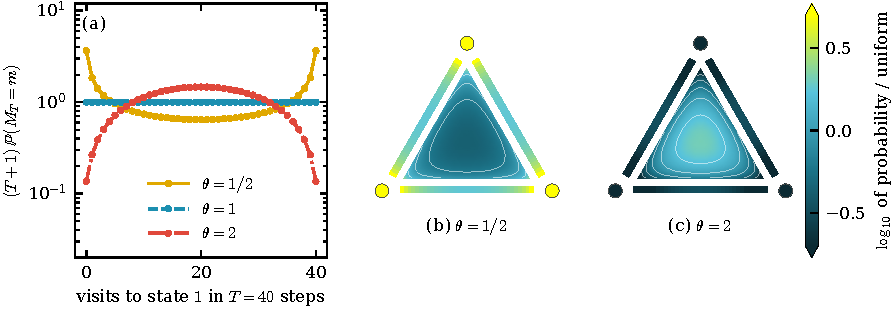
\includegraphics[width=\textwidth]{figures/aging}
\caption{The exact law~\eqref{eq:aging-urn} of the counts of the chain that
draws afresh or repeats. (a) Two states and $T=40$, as a multiple of the
uniform law. The law is flat at $\theta=1$, the ends are the most likely points
for $\theta=\frac12$, and the center is for $\theta=2$. (b), (c) Three states
and $T=36$ on the simplex of visit fractions, colored by the probability of a
count vector relative to the uniform law. The triangle holds the count vectors
that use all 3 states, the bands hold those that use 2, and the disks are
those that use 1. The thin lines are level lines. For $\theta=\frac12$ a corner is
$9.6$ times as likely as under the uniform law and the center $0.43$ times.
For $\theta=2$ the numbers are $0.035$ and $2.1$.}
\label{fig:aging}
\end{figure}

\begin{proof}
We use induction on $T$. For $T=1$ both sides of~\eqref{eq:aging-urn} are
$\frac1d$ when $m=e_j$ and $0$ otherwise. Let $T\ge2$ and suppose
\eqref{eq:aging-urn} holds for $T-1$. If $m_j=0$ both sides vanish. Otherwise
put $m'=m-e_j$. Summing~\eqref{eq:aging-urn} over the last state gives
$\Prob(M_{T-1}=m')=Q_{T-1}(m')$. A fresh draw gives $j$ with probability
$\frac1d$ whatever the last state was, and a repeat gives $j$ only when the
last state was $j$ (this is why the induction carries the last state along
with the counts). So
\[
 \Prob(M_T=m,\,Y_T=j)
 =\frac{f_T}{d}\,Q_{T-1}(m')+(1-f_T)\,\frac{m_j-1}{T-1}\,Q_{T-1}(m')
 =\frac{\theta+m_j-1}{d\theta+T-1}\,Q_{T-1}(m') .
\]
On the other hand
$Q_T(m)=Q_{T-1}(m')\cdot\frac{T}{m_j}\cdot\frac{\theta+m_j-1}{d\theta+T-1}$ by
the definition of $Q_T$. This gives~\eqref{eq:aging-urn}. Summing over $j$
gives $\Prob(M_T=m)=Q_T(m)$, and the ratio~\eqref{eq:aging-urn-ratio} is
$Q_T(T/2,T/2)/Q_T(T,0)$ with
$\theta^{(T)}=\theta^{(T/2)}(\theta+T/2)^{(T/2)}$. Each factor
$(\theta+i)/(\theta+T/2+i)$ increases strictly in $\theta$, and at
$\theta=1$ the product is $(T/2)!^2/T!$.
\end{proof}

The law of the counts alone is known. Dietz, Lippitt and
Sethuraman~\cite[Theorem~2.18]{dls2023} show that the moments of the limit
law of the chains of~\cite{ds2007} are occupation probabilities at finite $N$
of a second chain. In the case of a Dirichlet limit that second chain is
$Y$, with the uniform law in the role of their $\mu$ and $d\theta$ in the role
of their $\theta$. The limit is then the Dirichlet law with every parameter
$\theta$~\cite[Theorem~1.4]{ds2007}, and its moments give $Q_T$.
Engl\"ander and Volkov work it out in Chapter~7 of their
March 18, 2024 draft~\cite{ev2024}. For 2 states and an integer weight $\theta$
they prove~\eqref{eq:aging-urn}, with the last state, for every
$T$~\draftloc{Theorem~7.2, pp.~138--139}, and they credit this result to E.~Crane.
What the proposition adds is the joint law with the last state for $d\ge3$
states, and for a weight $\theta$ that is not an integer. As $T\to\infty$,
\eqref{eq:aging-urn} turns into the joint limit of the fractions of time and
the current state found by Bouguet and Cloez~\cite[Proposition~4.1]{bc2018},
in which the Dirichlet law is size-biased by the coordinate of the current
state.

\begin{remark}\label{rem:aging-feller}
Here is another way to see the law of the counts in
Proposition~\ref{prop:aging-urn} (but not the joint law with the last state).
The fresh draws
cut $Y_1,\dots,Y_T$ into runs, and each run gets a uniform state. The urn can
be run in the same way, as a Chinese restaurant process in which each table
gets a uniform color. There a table is opened with the same probabilities
$f_t$. The lengths of the runs are the spacings between the successes of
independent trials with success probabilities $f_t$. It is a classical
fact (the Feller coupling, see~\cite{abt2003}) that the multiset of these spacings has
the same law as the multiset of the table sizes (the two ordered lists do not).
The proof in~\draftloc{Section~7.4}, like
Proposition~\ref{prop:aging-urn}, instead goes through the last state. We
checked~\eqref{eq:aging-urn} in exact arithmetic for 4 values of $\theta$,
with $T\le7$ for $d=2,3$ and $T\le5$ for $d=4$
(\texttt{verify\_aging\_urn.py}).
\end{remark}

\subsection{A fixed first step}

Here the walk starts with a step $+1$.

\begin{proposition}[2 states, fixed first step]\label{prop:aging-two}
Let $N\ge2$ and let the first step be $+1$.
\begin{enumerate}[(a)]
\item At $c=1$, for $1\le s\le N$,
\[
 \Prob_+(A_N=s,\,X_N=+1)=\frac{s-1}{N(N-1)},\qquad
 \Prob_+(A_N=s,\,X_N=-1)=\frac{N-s}{N(N-1)}.
\]
So $A_N$ is uniform on $\{1,\dots,N\}$.
\item For $1\le s\le N-1$ the ratio $\Prob_+(A_N=s)/\Prob_+(A_N=N)$ increases
strictly in $c\in(0,2)$, and it equals $1$ exactly at $c=1$.
\end{enumerate}
\end{proposition}

For $c<1$ the end $N$ is the most likely value of $A_N$, and for $c>1$ it is
the least likely of the values $1,\dots,N$ (the value $0$ has probability
$0$).

\begin{proof}
(a) At $c=1$, the shifted chain $Y_t=X_{t+1}$ is the chain of
Proposition~\ref{prop:aging-urn} with $d=2$, $\theta=1$ and uniform first
state. Apply~\eqref{eq:aging-urn} at $T=N-1$ with counts $(s-1,N-s)$,
where $Q_{N-1}=1/N$, then sum over the last state.

(b) We write the ratio as a sum over paths. Only the path with every step
$+1$ has $A_N=N$, and it never switches. So $\Prob_+(A_N=N)$ is the first
product in~\eqref{eq:aging-path}, and dividing by it leaves
\begin{equation}\label{eq:aging-ratio}
 \frac{\Prob_+(A_N=s)}{\Prob_+(A_N=N)}
 =\sum_{x}\ \prod_{t:\,x_t\ne x_{t-1}}\omega_t ,
\end{equation}
where the sum is over the paths $x$ with $x_1=+1$ and $s$ steps equal to
$+1$. For example, for $N=3$ and $s=2$ the paths are $(+,+,-)$ and $(+,-,+)$,
and the ratio is $\omega_3+\omega_2\omega_3$. For $1\le s\le N-1$ there is
such a path, and each of them switches at least once. So the right side is a
sum of products of the $\omega_t$ with at least one factor each. Each
$\omega_t$ is positive and increases strictly in $c$, so the sum does too. By
(a) it equals $1$ at $c=1$.
\end{proof}

After a shift of one step, part (a) is the exercise
in~\cite[Section~3.1, footnote~1]{evw2020}. That footnote also says that the fact
can be related to P\'olya urns (the authors credit M.~Bal\'azs) and that a
more general connection of their model with P\'olya urns will appear in a
later paper.
That connection is developed in Chapter~7 of the dated draft, and after the same
shift part (a), with the last state, is~\draftloc{Claim~7.1}. So part (a)
is not new. What we add for
2 states is part (b), and the count law also follows
from~\cite[Theorem~2.18]{dls2023} (Section~\ref{sec:aging-urn}). Both parts of
Proposition~\ref{prop:aging-two} are also proved in Lean
(Section~\ref{sec:verify}).

\subsection{\texorpdfstring{$d$}{d} states}

The same thing happens for a chain on $d$ states that leaves its current
state for each other state at the same aging rate. Fix $d\ge2$ and $\theta$
with $0<\theta<d/(d-1)$. The chain $X_1,X_2,\dots$ on $\{1,\dots,d\}$ starts at
$X_1=1$. At step $k\ge2$ it moves to each of the other $d-1$ states with
probability $\theta/(k+d-2)$, and it stays with probability
$1-(d-1)\theta/(k+d-2)$. The condition on $\theta$ says that the probability
of staying is positive at every step $k\ge2$. Let
$L_N=(L_N(1),\dots,L_N(d))$ be the vector of visit counts, namely
$L_N(i)=\#\{k\le N:X_k=i\}$. Its values are the compositions
$n=(n_1,\dots,n_d)$ of $N$ into $d$ nonnegative parts with $n_1\ge1$. There
are $\binom{N+d-2}{d-1}$ of them (subtract one from $n_1$). The corner
$Ne_1$, where $e_i$ is the $i$-th unit vector, is the count vector of the
chain that never moves.

For such chains Dietz and Sethuraman~\cite[Theorem~1.4]{ds2007} proved that
the fractions of time converge in law to the Dirichlet law with every
parameter $\theta$, which is uniform on the simplex exactly at $\theta=1$.
Our step $k$ uses their transition matrix at time $n=k+d-2$, and the two
agree for $n\ge d+1$. Both chains redraw a uniform state with probability
$d\theta/n$. After the first common redraw they agree, so their fractions of
time have the same limit. At
$\theta=1$, part~(a) of the theorem below is an exact finite-$N$ form of this
limit.

\begin{theorem}[$d$ states]\label{thm:aging-d}
Let $d\ge2$, $0<\theta<d/(d-1)$ and $N\ge2$.
\begin{enumerate}[(a)]
\item At $\theta=1$, for every count vector $n$ and every state $j$,
\begin{equation}\label{eq:aging-d}
 \Prob(L_N=n,\,X_N=j)=\frac{n_j-\mathbf 1\{j=1\}}{(N-1)\binom{N+d-2}{d-1}} .
\end{equation}
So $L_N$ is uniform on its $\binom{N+d-2}{d-1}$ values, the corner included.
\item For every count vector $n\ne Ne_1$ the ratio $\Prob(L_N=n)/\Prob(L_N=Ne_1)$
increases strictly in $\theta$, and it equals $1$ exactly at $\theta=1$.
\end{enumerate}
\end{theorem}

In words, at $\theta=1$, given the counts, the
last state is distributed as the state at a uniformly chosen one of the steps
$2,\dots,N$ (the forced first visit to state $1$ is left out).
Below $\theta=1$ the corner is the most likely count vector, and above it the corner
is the least likely.

\begin{proof}
(a) At $\theta=1$, $X_2$ is uniform and $Y_t=X_{t+1}$ is the chain
of Proposition~\ref{prop:aging-urn}. Its count vector is $L_N-e_1$, and
$Q_{N-1}=1/\binom{N+d-2}{d-1}$. Formula~\eqref{eq:aging-urn} gives
\eqref{eq:aging-d}, and summing over $j$ gives the uniform law.

(b) A path $x\in\{1,\dots,d\}^N$ with $x_1=1$ has probability
$\prod_{k=2}^N\bigl(1-\frac{(d-1)\theta}{k+d-2}\bigr)$ times the product of
the odds
\[
 \omega^{(d)}_t=\frac{\theta/(t+d-2)}{1-(d-1)\theta/(t+d-2)}
 =\frac{\theta}{t+d-2-(d-1)\theta}
\]
over the times $t\ge2$ with $x_t\ne x_{t-1}$. The denominator is positive and
decreases in $\theta$, so each $\omega^{(d)}_t$ increases strictly in
$\theta$. Only the constant path has counts $Ne_1$. So
$\Prob(L_N=n)/\Prob(L_N=Ne_1)$ is the sum of the products of the odds over
the paths with counts $n$. For a count vector $n\ne Ne_1$ there is such a path, and
each of them moves at least once. Hence the ratio increases strictly in
$\theta$, and by (a) it equals $1$ at $\theta=1$.
\end{proof}

\begin{remark}\label{rem:aging-d}
For $d=2$ the chain switches at step $k$ with probability $\theta/k$, so
Theorem~\ref{thm:aging-d} with $\theta=c$ is
Proposition~\ref{prop:aging-two}, and~\eqref{eq:aging-d} reads
$(s-1)/(N(N-1))$ for $j=1$ and $n=(s,N-s)$.

By Proposition~\ref{prop:aging-urn}, $(L_N-e_1,X_N)$ has the law of
the counts and last color of $N-1$ draws from P\'olya's urn with one ball of
each color. This is an identity at each fixed time, not an identity of path
laws. For example, with $d=2$ and $N=4$ the chain path $1,1,2,2$ has
probability $1/8$, while the urn draws $1,2,2$ have probability $1/12$.
For 2 states Engl\"ander and Volkov call this relation
mimicking~\draftloc{Definition~7.1 and Lemma~7.1}, and they show with an
example of 3 steps that the coin-turning walk and the urn have different
path laws~\draftloc{Example~7.1}. Also, at $\theta=1$ the chain moves at
step $k$ with probability $(d-1)/(k+d-2)$, independently over $k$. This is
the probability that customer $k$ opens a new table in the Chinese restaurant
process with parameter $d-1$. So the expected number of moves in $N$ steps at
the tie is $\sum_{k=2}^N\frac{d-1}{k+d-2}=(d-1)\log N+O(1)$, which has the
same order, $\log N$, as the number of turns at the crossing from the corners
to the center for $d$ directions and runs of geometric length
(Section~\ref{sec:prior}).

We checked~\eqref{eq:aging-d}, and the strict ordering in (b) along the 5
values $\theta=\frac12,\frac9{10},1,\frac{11}{10},\frac54$, in exact
rational arithmetic for $d=2,3,4$ and $2\le N\le8$
(\texttt{verify\_aging.py}).
\end{remark}

\subsection{A fair first step}

We return to 2 states and let the first step be fair. Then both ends can be
reached, and $E_N=\Prob(A_N=N)=\frac12\prod_{k=2}^N(1-c/k)$. Changing the sign
of every step preserves the law of the walk and sends $A_N$ to $N-A_N$. So
\begin{equation}\label{eq:aging-fair}
 \Prob(A_N=s)=\tfrac12\bigl(\Prob_+(A_N=s)+\Prob_+(A_N=N-s)\bigr),\qquad
 E_N=\tfrac12\Prob_+(A_N=N),
\end{equation}
since $\Prob_+(A_N=0)=0$.

\begin{proposition}[fair first step]\label{prop:aging-fair}
Let $N\ge2$ and $1\le s\le N-1$, with a fair first step.
\begin{enumerate}[(a)]
\item At $c=1$, $\Prob(A_N=s)=\frac1N$ and $E_N=\frac1{2N}$.
\item The ratio $\Prob(A_N=s)/E_N$ is continuous and strictly increasing in
$c\in(0,2)$. It tends to $0$ as $c\downarrow0$ and equals $2$ at $c=1$. So
there is exactly one $c$ in $(0,2)$ with $\Prob(A_N=s)=E_N$, and it is less
than $1$.
\end{enumerate}
\end{proposition}

For even $N$ we write $c_N$ for the crossing in (b) with $s=h=N/2$, so that
$C_N=E_N$ exactly at $c=c_N$. In words, at $c=1$ every interior point still has
probability $\frac1N$, and the two ends share the probability $\frac1N$ that
the fixed start gave to one end.
Engl\"ander and Volkov give related fair-start formulas for switch
probabilities $1/(n+a)$~\draftloc{Section~5.7, p.~76}. We derive (a) from the
symmetry identity~\eqref{eq:aging-fair} instead.

\begin{proof}
(a) This follows from~\eqref{eq:aging-fair} and
Proposition~\ref{prop:aging-two}(a). (b) By~\eqref{eq:aging-fair} the ratio
is the sum of the right sides of~\eqref{eq:aging-ratio} for $s$ and for
$N-s$. Both are finite sums of products of at least one $\omega_t$. So the
ratio is continuous and strictly increasing, and it tends to $0$ as
$c\downarrow0$. By (a) it equals $2$ at $c=1$. Hence it equals $1$ exactly
once, at some $c<1$.
\end{proof}

How far below $1$ is $c_N$? The end is of order $N^{-c}$ and the center is of
order $1/N$, so they meet when $N^{1-c}$ is about $2$.

\begin{proposition}[the fair-start crossing]\label{prop:aging-expansion}
For even $N\to\infty$,
\[
 c_N=1-\frac{\log2}{\log N+\gamma+2-2\log2}+O\bigl((\log N)^{-3}\bigr),
\]
where $\gamma$ is Euler's constant.
\end{proposition}

\paragraph{Idea of the proof.}
A monotonicity argument first traps $c_N$ within $O(1/\log N)$ of $1$, so an expansion at $c=1$
applies. The end is explicit, namely
$E_N=\Gamma(N+1-c)/(2\Gamma(2-c)\Gamma(N+1))$, which is
$N^{-c}/(2\Gamma(2-c))$ with relative error $O(1/N)$. For the center we prove
a local limit theorem with a rate, namely $NC_N=d_c+O(\sqrt{\log N/N})$ uniformly
for $c\in[c^{(3)},1]$, where $c^{(3)}=(9-\sqrt{57})/2\approx0.725$ and $d_c=4^{1-c}/\mathrm B(c,c)$ is the density of
$\mathrm{Beta}(c,c)$ at $\frac12$. So
$\log(C_N/E_N)=(c-1)\log N+\Theta(c)+O(\sqrt{\log N/N})$ with
$\Theta(c)=\log(2\Gamma(2-c)d_c)$. Here $\Theta(1)=\log2$ and
$\Theta'(1)=\gamma+2-2\log2$, and solving for the zero gives the expansion.
The proof is in Appendix~\ref{app:aging}. There $C_N$ is an average of
explicit numbers over the law of the time of the $h$-th step $+1$
(Lemma~\ref{lem:D-average}). The local limit theorem comes from a coupling of
the walk with the chain of Proposition~\ref{prop:aging-urn} with $d=2$ and
$\theta=c$, whose counts are a mixture of binomial laws with a
$\mathrm{Beta}(c,c)$ parameter (Proposition~\ref{prop:D-llt}).

The error term decays only like $(\log N)^{-3}$, but the expansion is
already accurate at moderate $N$. The computed crossing at $N=200$ is
$c_{200}=0.8925$, against $0.8932$ from the expansion without its error term. The constant in
the error term is not computed.


\appendix
\section{Proof of Proposition~\ref{prop:aging-expansion}}\label{app:aging}

We bound a gamma ratio, bracket $C_N$ and $c_N$, prove a local limit theorem
at the center, and then expand the crossing. We use the setting of
Sections~\ref{sec:notation} and~\ref{sec:aging} with 2 states and a fair first step. So $0<c<2$, $X_1$ is a fair sign, and the switch indicators
$\chi_k=\mathbf 1\{X_k\ne X_{k-1}\}$, $k\ge2$, are independent
Bernoulli$(c/k)$ variables, independent of $X_1$. Put
\[
\rho(a,b)=\prod_{k=a+1}^{b}\Bigl(1-\frac ck\Bigr)
=\frac{\Gamma(b+1-c)\,\Gamma(a+1)}{\Gamma(b+1)\,\Gamma(a+1-c)},\qquad
\lambda_{t,N}=\frac ct\,\rho(t,N)
\]
for integers $1\le a\le b$ and $2\le t\le N$. So $\lambda_{t,N}$ is the
probability of a switch at time $t$ and none in $(t,N]$, and
$E_N=\frac12\rho(1,N)$. Let $T^+_s$ be the time of the $s$-th step equal to
$+1$. Let $B$ be a Beta$(c,c)$ variable, $d_c=4^{1-c}/\mathrm B(c,c)$ its
density at $\frac12$, and $\Theta(c)=\log\bigl(2\Gamma(2-c)\,d_c\bigr)$. For
even $N$ we write $h=N/2$ and $C_N=\Prob(A_N=h)$. Changing the sign of every
step preserves the law of the walk and sends $A_N$ to $N-A_N$. We call this
flip symmetry.

\subsection{A gamma ratio}

Gautschi's inequality~\cite[5.6.4]{dlmf} says that
$x^{1-s}<\Gamma(x+1)/\Gamma(x+s)<(x+1)^{1-s}$ for $x>0$ and $0<s<1$. We
claim that for $0<c<2$ and real $y\ge2$,
\begin{equation}\label{eq:D-gamma}
\frac{\Gamma(y+1-c)}{\Gamma(y+1)}=y^{-c}(1+\vartheta)\qquad\text{with}\qquad
-\frac1y\le\vartheta\le\frac2y .
\end{equation}
If $c=1$ the left side is $1/y$ and $\vartheta=0$. If $c<1$ we take $x=y$ and
$s=1-c$. Then the left side lies between $(y+1)^{-c}$ and $y^{-c}$, and
$(1+1/y)^{-c}\ge1-c/y\ge1-1/y$. If $c>1$ we take $x=y$ and $s=2-c$ and use
$\Gamma(y+1-c)=\Gamma(y+2-c)/(y+1-c)$. Then the left side lies between
$(y+1)^{1-c}/(y+1-c)$ and $y^{1-c}/(y+1-c)$. Here
$y/(y+1-c)=1+(c-1)/(y+1-c)\le1+1/(y-1)\le1+2/y$, and
$(1+1/y)^{1-c}\,y/(y+1-c)\ge(1+1/y)^{-1}\ge1-1/y$.

\subsection{Averaging at the center and a bracket}

\begin{lemma}[averaging at the center]\label{lem:D-average}
Let $N\ge2$ be even and $T=T^+_h$. Then
\begin{equation}\label{eq:D-average}
C_N=2\sum_{r=h}^{N-1}\Prob(T=r)\,\lambda_{r+1,N}\qquad\text{and}\qquad
\sum_{r=h}^{N-1}\Prob(T=r)=\frac12 .
\end{equation}
If $0<c\le1$, then $c/N\le C_N\le\lambda_{h+1,N}$.
\end{lemma}

\begin{proof}
On the event $\{A_N=h,\,X_N=-1\}$ the last step equal to $+1$ is the $h$-th
one, at a time $T=r\le N-1$. It is followed by a switch at $r+1$ and no switch
in $(r+1,N]$. Conversely, these conditions give $A_N=h$ and $X_N=-1$. The
event $\{T=r\}$ depends only on $X_1,\chi_2,\dots,\chi_r$. So
$\Prob(A_N=h,\,X_N=-1)=\sum_{r=h}^{N-1}\Prob(T=r)\,\lambda_{r+1,N}$, and flip
symmetry gives the same value for $X_N=+1$. Next, $T\le N-1$ exactly when
$A_{N-1}\ge h$. This has probability $\frac12$, because $N-1$ is odd and
$A_{N-1}$ is symmetric about $(N-1)/2$. Finally
$\lambda_{t+1,N}/\lambda_{t,N}=t/(t+1-c)$, which is at most $1$ for $c\le1$.
So $\lambda_{N,N}=c/N\le\lambda_{t,N}\le\lambda_{h+1,N}$ for
$h+1\le t\le N$, and by~\eqref{eq:D-average} $C_N$ is a weighted average of
these values.
\end{proof}

For an integer $M\ge2$ put $\eta_M(c)=M\rho(1,M)/(2c)$. Since $\rho(1,M)$
decreases in $c$ and equals $1/M$ at $c=1$, the function $\eta_M$ decreases
strictly on $(0,1]$, from $\infty$ at $0$ to $\eta_M(1)=\frac12$. Let
$c^{(M)}\in(0,1)$ be the root of $\eta_M=1$.

\begin{proposition}[bracket]\label{prop:D-bracket}
The numbers $c^{(M)}$ increase with $M$, and
$1-c^{(M)}=\frac{\log2}{\log M+1+\gamma}+O\bigl((\log M)^{-3}\bigr)$. For
every even $N\ge2$ we have $c^{(h+1)}\le c_N\le c^{(N)}$. So
$(1-c_N)\log N\to\log2$, and $c_N\ge c^{(3)}=(9-\sqrt{57})/2>0.725$ for
$N\ge4$.
\end{proposition}

\begin{proof}
The equation $\eta_M(c)=1$ says that $\frac12\rho(1,M)=c/M$, namely that the
end for $M$ steps equals $c/M$. We compare $E_N$ with the 2 bounds for $C_N$
in Lemma~\ref{lem:D-average}, and each comparison is an inequality for some
$\eta_M$.

\emph{Monotonicity.} For $c<1$ we have $\eta_{M+1}/\eta_M=(M+1-c)/M>1$. So
$\eta_{M+1}(c^{(M)})>1$, and since $\eta_{M+1}$ decreases, $c^{(M+1)}>c^{(M)}$.

\emph{The bracket.} By Proposition~\ref{prop:aging-fair}(b), $C_N<E_N$ for
$c<c_N$ and $C_N>E_N$ for $c>c_N$, and $c_N<1$. So it is enough to compare
$C_N$ with $E_N$ for $0<c<1$. Let $c^{(N)}<c<1$. Then $\eta_N(c)<1$, that is
$E_N=\frac12\rho(1,N)<c/N$, and $c/N\le C_N$ by Lemma~\ref{lem:D-average}. So
$C_N>E_N$, which means $c>c_N$. Hence $c_N\le c^{(N)}$. Now let
$c<c^{(h+1)}$. Then $\eta_{h+1}(c)>1$, that is
$\frac12\rho(1,h+1)>c/(h+1)$. With $\rho(1,N)=\rho(1,h+1)\rho(h+1,N)$ this
gives $E_N>\frac{c}{h+1}\rho(h+1,N)=\lambda_{h+1,N}\ge C_N$. So $c<c_N$.
Hence $c_N\ge c^{(h+1)}$.

\emph{The expansion.} The number $c^{(3)}$ solves
$3\rho(1,3)=(2-c)(3-c)/2=2c$, that is $c^2-9c+6=0$. For $N\ge4$ we have
$h+1\ge3$, so $c_N\ge c^{(h+1)}\ge c^{(3)}$. By~\eqref{eq:D-gamma} with $y=M$
we have $M\rho(1,M)=M^{1-c}(1+O(1/M))/\Gamma(2-c)$. So the equation
$\eta_M(c)=1$ reads $(1-c)\log M=\Theta_0(c)+O(1/M)$ with
$\Theta_0(c)=\log\bigl(2c\,\Gamma(2-c)\bigr)$, uniformly for $0<c\le1$. For
$M\ge3$ we have $c^{(M)}\in[c^{(3)},1)$, where $\Theta_0$ is bounded. So
$\varepsilon=1-c^{(M)}$ is $O(1/\log M)$, and we may expand at $c=1$. We have
$\Theta_0(1)=\log2$ and $\Theta_0'(1)=1-\psi(1)=1+\gamma$, where
$\psi=\Gamma'/\Gamma$ and $\psi(1)=-\gamma$~\cite[5.4.12]{dlmf}. Taylor's
theorem gives
$\varepsilon(\log M+1+\gamma)=\log2+O(\varepsilon^2)+O(1/M)$, which is the
expansion. The limit
of $(1-c_N)\log N$ follows since $\log(h+1)\sim\log N$.
\end{proof}

\subsection{A local limit at the center}

\begin{proposition}[local limit at the center]\label{prop:D-llt}
For each compact $J\subset(0,2)$ there is $C_J$ such that
$\bigl\lvert NC_N-d_c\bigr\rvert\le C_J\sqrt{\log N/N}$ for $c\in J$
and even $N\ge4$.
\end{proposition}

\begin{proof}
We start from the averaging identity of Lemma~\ref{lem:D-average} and replace
the law of $T=T^+_h$ by its continuum version. Since $T\le r$ exactly when
$A_r\ge h$, we need the law of $A_r$. The chain of
Proposition~\ref{prop:aging-urn} with $d=2$ and $\theta=c$ switches with
nearly the same probabilities as the walk, and its counts are binomial with a
random parameter $B$. So $A_r$ is close in law to $rB$, and the time $T$ is
close in law to $h/B$. The weights $\lambda_{r+1,N}$ are explicit, so the
average becomes an explicit integral against the Beta$(c,c)$ density.

The proof has 5 steps. Step~1 shows that the counts of the chain are
binomial with the random parameter $B$. Step~2 couples the walk with the chain
and bounds the difference of the distribution functions of $T$ and $h/B$. Step~3 uses
summation by parts to replace the law of $T$ by that of $h/B$ in the average.
Step~4 writes the new sum as an expectation over $B$, and Step~5 evaluates it.

Let $F(r)=\Prob(T\le r)=\Prob(A_r\ge h)$, $\Phi(r)=\Prob(rB\ge h)$ and
$\Lambda_r=N\lambda_{r+1,N}$. By Lemma~\ref{lem:D-average},
\[
NC_N=2\sum_{r=h}^{N-1}\bigl(F(r)-F(r-1)\bigr)\Lambda_r .
\]
In this proof $C$ depends only on $J$ and may change from line to line. Since
$NC_N\le N$ and $d_c$ is bounded on $J$, it is enough to prove the claim for
large $N$. We put $K=\lceil\sqrt N\rceil$, $u=\sqrt{N\log N}$ and $w=K+u$, and
we take $N$ so large that $w\le h/4$. Note that $K\le h$.

\emph{Step 1 (a chain with binomial counts).} Let $X'$ be the chain of
Proposition~\ref{prop:aging-urn} with $d=2$ and $\theta=c$, written with the
states $\pm1$, and let $A'_r$ be its number of steps $+1$ among the first $r$.
Its first step is a fair sign, and at step $k\ge2$ it switches with
probability $q_k=c/(k-1+2c)$, independently of the past. By
Proposition~\ref{prop:aging-urn} and $x^{(m)}=\Gamma(x+m)/\Gamma(x)$,
\[
\Prob(A'_r=s)=\binom rs\frac{c^{(s)}c^{(r-s)}}{(2c)^{(r)}}
=\binom rs\frac{\mathrm B(c+s,c+r-s)}{\mathrm B(c,c)}
=\E\Bigl[\binom rsB^s(1-B)^{r-s}\Bigr].
\]
So $A'_r$ has the law of a binomial variable with $r$ trials and the random
success probability $B$. By Hoeffding's inequality~\cite[Theorem~1]{hoeffding1963},
a binomial variable with $r$ trials and success probability $x$ is at least
$rx+u$ with probability at most $e^{-2u^2/r}$, and the same holds for being at
most $rx-u$. Hence for every real $y$
\[
\Prob(rB\ge y+u)-e^{-2u^2/r}\le\Prob(A'_r\ge y)\le\Prob(rB\ge y-u)+e^{-2u^2/r}.
\]

\emph{Step 2 (coupling the walk with $X'$).} The switch probabilities differ
by $c/k-q_k=c(2c-1)/(k(k-1+2c))$, which is at most $6/(k(k-1))$ in absolute
value since $c<2$. Let $K\le r\le N$. For $K<k\le r$ we couple the switch
indicator $\chi_k$ of the walk with the switch indicator $\chi'_k$ of $X'$ so
that $\Prob(\chi_k\ne\chi'_k)=\lvert c/k-q_k\rvert$, using independent extra
randomness. We put $X_K=X'_K$ and $X_k=X_{k-1}(-1)^{\chi_k}$ for $K<k\le r$,
and we draw $X_1,\dots,X_{K-1}$ from the law of the walk given $X_K$, again
with independent randomness. In both processes the sign at step $K$ is fair,
and the later switches are independent of the first $K$ steps. So
$(X_1,\dots,X_r)$ has the law of the walk. Outside an event of probability at
most $\sum_{k>K}6/(k(k-1))=6/K$ the two processes agree at the steps
$K,\dots,r$, and then $\lvert A_r-A'_r\rvert<K$. With Step 1, $w=K+u$ and
$e^{-2u^2/r}\le e^{-2\log N}$, this gives
\[
\lvert F(r)-\Phi(r)\rvert\le\Prob(h-w\le rB<h+w)+\frac1{N^2}+\frac6K
\qquad(K\le r\le N).
\]

\emph{Step 3 (replacing $F$ by $\Phi$).} Put $\Delta(r)=F(r)-\Phi(r)$. Then
$\Delta(h-1)=0$, because $A_{h-1}<h$ and $B<1$. Summation by parts gives
\[
\sum_{r=h}^{N-1}\bigl(\Delta(r)-\Delta(r-1)\bigr)\Lambda_r
=\Delta(N-1)\Lambda_{N-1}-\sum_{r=h}^{N-2}\Delta(r)\bigl(\Lambda_{r+1}-\Lambda_r\bigr).
\]
The ratio $\lambda_{t+1,N}/\lambda_{t,N}=t/(t+1-c)$ gives
$\Lambda_{r+1}-\Lambda_r=\Lambda_r(c-1)/(r+2-c)$. Every factor of
$\rho(r+1,N)$ lies in $(0,1)$, so $\Lambda_r=\frac{Nc}{r+1}\rho(r+1,N)\le2c$
for $r\ge h$. Hence $\Lambda_{N-1}=c$ and
$\lvert\Lambda_{r+1}-\Lambda_r\rvert\le2c/h\le8/N$, and the right side is at
most $c\lvert\Delta(N-1)\rvert+\frac8N\sum_{r=h}^{N-2}\lvert\Delta(r)\rvert$
in absolute value. For each value $b$ of $B$ the number $rb$ lies in
$[h-w,h+w)$ for at most $2w/b+1$ integers $r$, and for no $r\le N$ unless
$b\ge(h-w)/N\ge\frac38$. So the probabilities in Step 2 add up to at most
$6w+1$ over $r$, and
$\sum_{r=h}^{N-2}\lvert\Delta(r)\rvert\le6w+2+3\sqrt N$. For $r=N-1$ the
event in Step 2 puts $B$ in an interval of length $2w/(N-1)$ inside
$[\frac38,\frac34]$, where the density of $B$ is at most $C$ for $c\in J$. So
$\lvert\Delta(N-1)\rvert\le Cw/N+N^{-2}+6/K$. Together, replacing $F$ by
$\Phi$ changes $NC_N$ by at most $C(w/N+1/K)\le C\sqrt{\log N/N}$.

\emph{Step 4 (the new sum is an expectation).} After the replacement the sum
is
\[
 2\sum_{r=h}^{N-1}\bigl(\Phi(r)-\Phi(r-1)\bigr)\Lambda_r .
\]
The term with $r=h$
vanishes, since $\Phi(h)=\Phi(h-1)=0$. For $h<r\le N-1$ we have
$\Phi(r)-\Phi(r-1)=\Prob(h/r\le B<h/(r-1))$, and on this event
$\lceil h/B\rceil=r$. These events are disjoint, and their union is
$\{h/(N-1)\le B<1\}$. So the new sum is
$2\,\E\bigl[\Lambda_{\lceil h/B\rceil};\,B\ge h/(N-1)\bigr]$.

\emph{Step 5 (evaluating the expectation).} By~\eqref{eq:D-gamma} with $y=N$
and $y=r+1\ge3$,
$\Lambda_r=c\bigl((r+1)/N\bigr)^{c-1}(1+O(1/N))$ for $h\le r\le N-1$. On the
event above with $r=\lceil h/B\rceil$, the number $(r+1)/N$ lies in
$[\frac12,2]$ and within $2/N$ of $h/(BN)=1/(2B)$, which also lies in
$[\frac12,2]$. The function $x^{c-1}$ is $4$-Lipschitz on $[\frac12,2]$. So
$\Lambda_{\lceil h/B\rceil}=c(2B)^{1-c}+O(1/N)$. Also
$\Prob\bigl(\frac12\le B<h/(N-1)\bigr)=O_J(1/N)$, since the density of $B$ is
bounded near $\frac12$ uniformly on $J$. So we may replace the event
$\{B\ge h/(N-1)\}$ by $\{B\ge\frac12\}$. In the remaining integral the factor
$b^{1-c}$ cancels the factor $b^{c-1}$ of the density. Hence, by Step 3,
$NC_N$ is within $C\sqrt{\log N/N}$ of
\[
2c\,\E\bigl[(2B)^{1-c};\,B\ge\tfrac12\bigr]+O_J(1/N)
=\frac{2c\,2^{1-c}}{\mathrm B(c,c)}\int_{1/2}^1(1-b)^{c-1}\,db+O_J(1/N)=d_c+O_J(1/N).\qedhere
\]
\end{proof}

\subsection{The expansion of the crossing}

\begin{proof}[Proof of Proposition~\ref{prop:aging-expansion}]
We write $\log C_N-\log E_N$ as an explicit function of $c$ with a small
error, and we solve for its zero near $c=1$. Let $J=[c^{(3)},1]$. Then $d_c$ is
bounded below on $J$ by a positive constant. By~\eqref{eq:D-gamma} with
$y=N$,
$\log E_N=\log\bigl(\tfrac12\rho(1,N)\bigr)=-\log2-\log\Gamma(2-c)-c\log N+O(1/N)$.
By Proposition~\ref{prop:D-llt},
$\log C_N=\log d_c-\log N+O(\sqrt{\log N/N})$ for large $N$. Both hold uniformly for
$c\in J$, so
\begin{equation}\label{eq:D-logratio}
\log C_N-\log E_N=(c-1)\log N+\Theta(c)+O(\sqrt{\log N/N})\qquad(c\in J).
\end{equation}
Here $\Theta(1)=\log2$ because $d_1=1$. Next,
$\Theta'(c)=-\psi(2-c)-\log4-2\psi(c)+2\psi(2c)$, and with $\psi(1)=-\gamma$
and $\psi(2)=1-\gamma$~\cite[5.4.12, 5.4.14]{dlmf} this gives
$\Theta'(1)=\gamma+2-2\log2$. Put
$L=\log N+\Theta'(1)$. By Proposition~\ref{prop:D-bracket}, $c_N\in J$ for
$N\ge4$ and $\varepsilon=1-c_N$ is $O(1/\log N)$. The left side
of~\eqref{eq:D-logratio} vanishes at $c=c_N$, because $C_N=E_N$ there. As
$\Theta$ is smooth on $J$, Taylor's theorem gives
$\Theta(c_N)=\log2-\varepsilon\,\Theta'(1)+O(\varepsilon^2)$.
So~\eqref{eq:D-logratio} at $c=c_N$ reads
$0=-\varepsilon\log N+\log2-\varepsilon\,\Theta'(1)+O(\varepsilon^2)+O(\sqrt{\log N/N})$,
that is
$\varepsilon L=\log2+O(\varepsilon^2)+O(\sqrt{\log N/N})=\log2+O(L^{-2})$. So
$\varepsilon=\log2/L+O(L^{-3})$, which is the expansion.
\end{proof}

With one more term in Taylor's theorem and
$\varepsilon^2=(\log2)^2/L^2+O(L^{-4})$, the same argument adds the term
$-\Theta''(1)(\log2)^2/(2L^3)$ to the expansion of $c_N$, with error
$O(L^{-4})$. Here $\Theta''(1)=\pi^2/2-4$, since
$\Theta''(c)=\psi'(2-c)-2\psi'(c)+4\psi'(2c)$, $\psi'(1)=\zeta(2)$ and
$\psi'(2)=\zeta(2)-1$~\cite[5.4.12, 5.15.5]{dlmf}. At $N=200$ the bracket of
Proposition~\ref{prop:D-bracket} is $[0.88749,0.89878]$,
Proposition~\ref{prop:aging-expansion} gives $0.89319$, and with the $L^{-3}$
term we get $0.89236$. The high-precision value is $c_{200}=0.89253$. The
constants $C_J$ and the constants in the $O$-terms of this appendix are not
computed. Numerically $\lvert NC_N-d_c\rvert$ decays like $1/N$. At $c=0.75$
it drops by a factor of about $4$ each time $N$ is multiplied by $4$, from
$N=400$ to $N=6400$. So the rate in Proposition~\ref{prop:D-llt} is probably
not sharp.


\begin{thebibliography}{99}\small\setlength{\baselineskip}{11pt}\setlength{\itemsep}{0pt}\setlength{\parsep}{0pt}

\bibitem{kagey131}
Kagey, P.: Problem 131. Open Problem Collection.
\url{https://peterkagey.com/problems/131/}. Accessed October 2026

\bibitem{paperA}
Pemmasani, A.: Uniform Bessel bounds for magnetization crossings in finite
Ising chains. Preprint at \url{https://arxiv.org/abs/2610.06935} (2026)

\bibitem{paperB}
Pemmasani, A.: Vertex crossings in a symmetric Markov multinomial model.
Preprint at \url{https://arxiv.org/abs/2610.09258} (2026)

\bibitem{godrecheluck2001}
Godr\`eche, C., Luck, J.M.: Statistics of the occupation time of renewal
processes. J. Stat. Phys. \textbf{104}(3--4), 489--524 (2001).
\url{https://doi.org/10.1023/A:1010364003250}. Section and equation numbers
refer to arXiv:cond-mat/0010428v1

\bibitem{dlmf}
Olver, F.W.J., et al. (eds.): NIST Digital Library of Mathematical Functions.
Section~5.4(iii) and Eqs.~5.4.12, 5.4.14, 5.6.4 and~5.15.5.
\url{https://dlmf.nist.gov}

\bibitem{ds2007}
Dietz, Z., Sethuraman, S.: Occupation laws for some time-nonhomogeneous
Markov chains. Electron. J. Probab. \textbf{12}, 661--683 (2007).
\url{https://doi.org/10.1214/EJP.v12-413}. Example and theorem numbers refer
to arXiv:math/0701798v1

\bibitem{ev2018}
Engl\"ander, J., Volkov, S.: Turning a coin over instead of tossing it. J.
Theor. Probab. \textbf{31}(2), 1097--1118 (2018).
\url{https://doi.org/10.1007/s10959-016-0725-1}. Theorem numbers refer to
arXiv:1606.03281v1

\bibitem{abt2003}
Arratia, R., Barbour, A.D., Tavar\'e, S.: Logarithmic Combinatorial
Structures: A Probabilistic Approach. EMS Monographs in Mathematics. European
Mathematical Society, Z\"urich (2003). \url{https://doi.org/10.4171/000}

\bibitem{bc2018}
Bouguet, F., Cloez, B.: Fluctuations of the empirical measure of freezing
Markov chains. Electron. J. Probab. \textbf{23}, 2 (2018).
\url{https://doi.org/10.1214/17-EJP130}. Proposition numbers refer to
arXiv:1705.02121v1

\bibitem{dls2023}
Dietz, Z., Lippitt, W., Sethuraman, S.: Stick-breaking processes, clumping,
and Markov chain occupation laws. Sankhy\=a A \textbf{85}(1), 129--171
(2023). \url{https://doi.org/10.1007/s13171-020-00236-x}. Theorem numbers
refer to arXiv:1901.08135v1

\bibitem{ev2022}
Engl\"ander, J., Volkov, S.: Conservative random walk. Electron. J. Probab.
\textbf{27}, 138 (2022). \url{https://doi.org/10.1214/22-EJP863}

\bibitem{ev2024}
Engl\"ander, J., Volkov, S.: Coin-Turning, Random Walks and Inhomogeneous
Markov Chains. Author draft of March 18, 2024.
\url{https://www.researchgate.net/publication/379333206_Coin-Turning_Random_Walks_and_Inhomogeneous_Markov_Chains}.
Chapter, section, theorem and page numbers in this note refer to this draft.
We did not check them against the published edition~\cite{ev2025}

\bibitem{ev2025}
Engl\"ander, J., Volkov, S.: Coin-Turning, Random Walks and Inhomogeneous
Markov Chains. World Scientific, Singapore (2025).
\url{https://doi.org/10.1142/13837}

\bibitem{evw2020}
Engl\"ander, J., Volkov, S., Wang, Z.: The coin-turning walk and its scaling
limit. Electron. J. Probab. \textbf{25}, 3 (2020).
\url{https://doi.org/10.1214/19-EJP406}

\bibitem{hoeffding1963}
Hoeffding, W.: Probability inequalities for sums of bounded random variables.
J. Am. Stat. Assoc. \textbf{58}(301), 13--30 (1963).
\url{https://doi.org/10.1080/01621459.1963.10500830}

\bibitem{prr2026}
Pradhan, A., Roy, R., Ray, P.: Diffusive-to-ballistic transition in a
persistent random walk. Preprint at \url{https://arxiv.org/abs/2605.20116}
(2026)

\end{thebibliography}


\begin{acks}[Acknowledgments]
I thank Peter Kagey, whose Problem~131 in his Open Problem
Collection~\cite{kagey131} started this work.
\end{acks}

\end{document}
